% Chapter 2

\chapter{Θεωρητικό Υπόβαθρο} % Main chapter title

\label{Chapter2} % For referencing the chapter elsewhere, use \ref{Chapter2} 
%----------------------------------------------------------------------------------------

% Define some commands to keep the formatting separated from the content 


%----------------------------------------------------------------------------------------

Σε αυτό το κεφάλαιο, θα δώσουμε κάποιους ορισμούς, για έννοιες που θα παρουσιαστούν αργότερα στα πλαίσια της εργασίας.


\section{Χρονοσειρές}

Χρονοσειρά ορίζεται ως μία ακολουθία από παρατηρήσεις, οι οποίες συλλέγονται ανά κανονικά/ακανόνιστα χρονικά διαστήματα, είναι διατεταγμένες σε χρονική σειρά, και λαμβάνονται από ιατρικά, οικονομικά, IoT, αισθητήρες, κ.ο.κ. Μπορεί να είναι μονοδιάστατες ή πολυδιάστατες, ανάλογα με τον αριθμό των μεταβλητών της κάθε μέτρησης. Στα πλαίσια της εργασίας θα ασχοληθούμε μόνο με μονοδιάστατες χρονοσειρές.

Συγκεκριμένα σύμφωνα με το \cite[Section 3.1]{schmidl2024autotsad}, ως μονοδιάστατες χρονοσειρές $T \in \mathrm{R}^n$ ορίζεται μία ακολουθία αληθινών μετρήσεων $T_i \in \mathrm{R}$, όπου $i \in |T|$ και $|T| = n$. Το μήκος της χρονοσειράς $T$ είναι $|T|$ ή $n$ και το i-οστό σημείο της ακολουθίας συμβολίζεται ως $T_i$.

%----------------------------------------------------------------------------------------

\section{Ανωμαλίες}

\emph{Ανωμαλίες} σε χρονοσειρές σύμφωνα με το \cite[Section 3.1]{paparrizos2022tsb}, ορίζονται ως σημεία, ή ακολουθίες σημείων, όπου αποκλίνουν σημαντικά από την κανονική συμπεριφορά της ακολουθίας, ή μίας υπακολουθίας της. Μπορεί να οφείλονται σε εσφαλμένες μετρήσεις ή σε πραγματικά ασυνήθιστα γεγονότα. Χωρίζονται σε τρεις κατηγορίες:
\begin{itemize}
    \item \emph{\bf{Point Anomalies}}: Αφορούν μεμονωμένα σημεία τα οποία διαφέρουν σημαντικά από τα υπόλοιπα σημεία της χρονοσειράς.
    \item \emph{\bf{Contextual Anomalies}}: Αφορούν σημεία, τα οποία μπορεί να είναι φυσιολογικά σε σχέση με τα υπόλοιπα σημεία της χρονοσειράς, αλλά να διαφέρουν σημαντικά δεδομένου ενός συγκεκριμένου πλαισίου.
    \item \emph{\bf{Collective anomalies}}: Αφορούν ακολουθίες σημείων, τα οποία δεν επαναλαμβάνουν ένα κανονικό, παρατηρήσιμο μοτίβο. Αξίζει να σημειωθεί, πως αν τα σημεία της υπακολουθίας παρατηρηθούν ως μεμωνομένα, μπορεί να ανιχνευτούν ως κανονικά από έναν αλγόριθμο ανίχνευσης ανωμαλιών.
\end{itemize}

\begin{figure}[h]
    \centering
    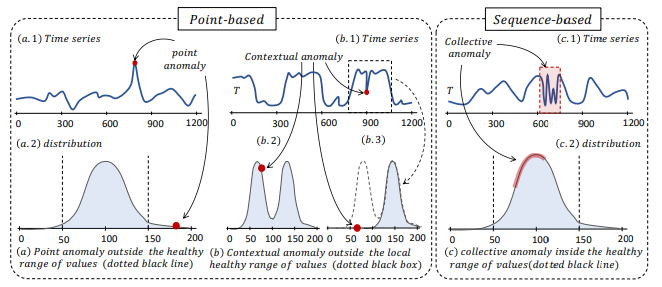
\includegraphics[width=1\linewidth]{Figures/anomalies_types.png}
    \caption{Τύποι ανωμαλιών σε χρονοσειρές (αναπαραγωγή από \cite{paparrizos2022tsb})}
    \label{figure:anomalies_types}
\end{figure}

Οι δημιουργοί του \emph{GutenTAG}\cite{10.14778/3554821.3554873} (βιβλιοθήκη για δημιουργία τεχνιτών χρονοσειρών με ή χωρίς ανωμαλίες), τις κατατάσουν στις εξής κατηγορίες:

\begin{itemize}
    \item \strong{Amplitude}: Αφορά στην αλλαγή του πλάτους του σήματος για κάποια χρονική περίοδο (Σχήμα \ref{figure:amplitude}).
    \begin{figure}[h]
    \centering
    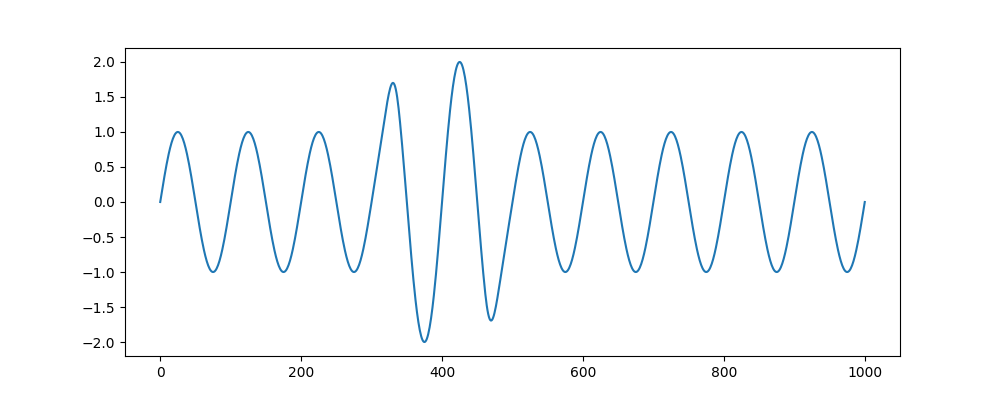
\includegraphics[width=1\linewidth]{Figures/gutenTAG_anomalies/amplitude.png}
    \caption{Amplitude anomaly (αναπαραγωγή από \cite{10.14778/3554821.3554873})}
    \label{figure:amplitude}
    \end{figure}
    \item  \strong{Extremum}: Αφορά την εμφάνιση μίας ακράια τιμής (spike) στο σήμα, το οποίο μπορεί να είναι είτε τοπικά μέγιστο-ελάχιστο, ή καθολικά μέγιστο-ελάχιστο (Σχήμα \ref{figure:extremum}).
    \begin{figure}[h]
    \centering
    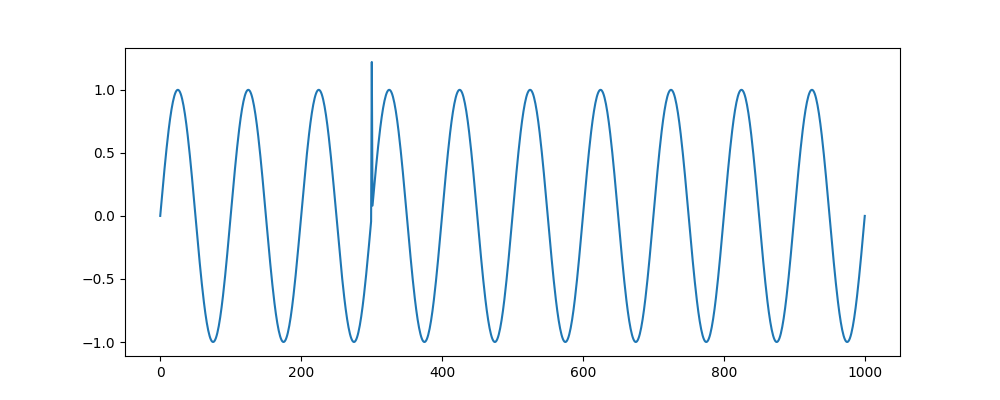
\includegraphics[width=1\linewidth]{Figures/gutenTAG_anomalies/extremum.png}
    \caption{Extremum anomaly (αναπαραγωγή από \cite{10.14778/3554821.3554873})}
    \label{figure:extremum}
    \end{figure}
    \item \strong{Συχνότητας}: Αφορά στην αλλαγή της συχνότητας σε μία χρονική περίοδο ενός σήματος (Σχήμα \ref{figure:frequency}).
    \begin{figure}[h]
    \centering
    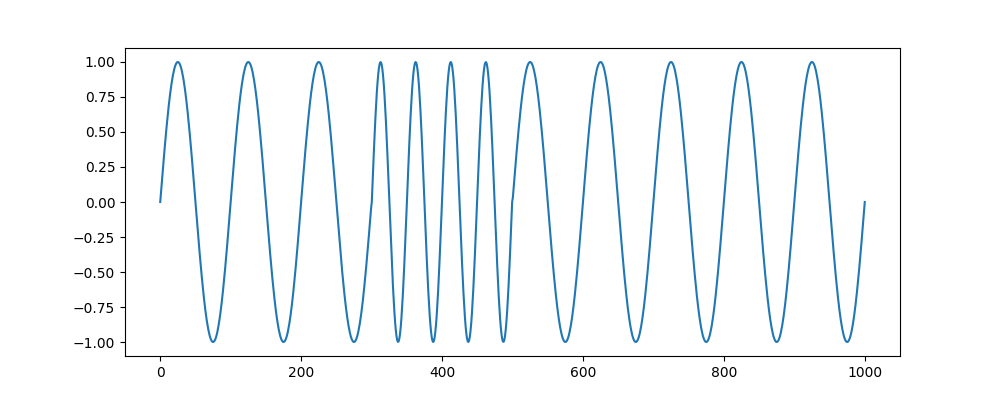
\includegraphics[width=1\linewidth]{Figures/gutenTAG_anomalies/frequency.png}
    \caption{Frequency anomaly (αναπαραγωγή από \cite{10.14778/3554821.3554873})}
    \label{figure:frequency}
    \end{figure}
    \item \strong{Mean}: Αφορά την κατακόρυφη μετατόπιση της χρονοσειράς κατά μία σταθερή τιμή για το διάστημα της ανωμαλίας (Σχήμα \ref{figure:mean}).
    \begin{figure}[h]
    \centering
    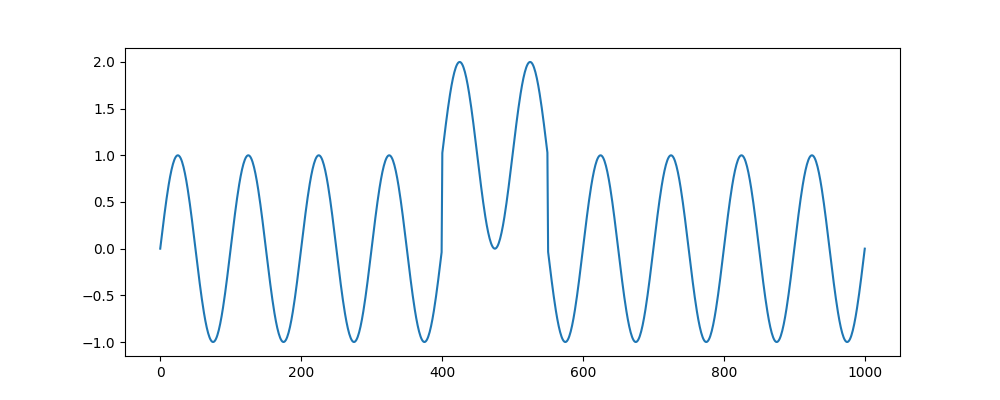
\includegraphics[width=1\linewidth]{Figures/gutenTAG_anomalies/mean.png}
    \caption{Mean anomaly (αναπαραγωγή από \cite{10.14778/3554821.3554873})}
    \label{figure:mean}
    \end{figure}
    \item \strong{Pattern}: Αφορά στην αλλαγή του επαναλαμβανόμενου μοτίβου της χρονοσειράς (π.χ. ένα ημιτονοειδές σήμα θα μπορούσε να παραμορφωθεί για το διάστημα της ανωμαλίας) (Σχήμα \ref{figure:pattern-ecg} και \ref{figure:pattern-shift}).
    \begin{figure}[h]
    \centering
    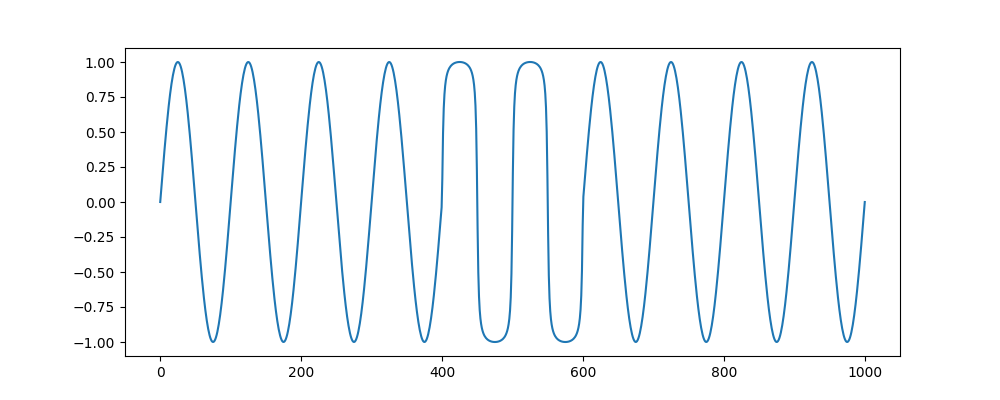
\includegraphics[width=1\linewidth]{Figures/gutenTAG_anomalies/pattern-sine.png}
    \caption{Pattern-sine anomaly (αναπαραγωγή από \cite{10.14778/3554821.3554873})}
    \label{pattern-sine}
    \end{figure}
    \begin{figure}[h]
    \centering
    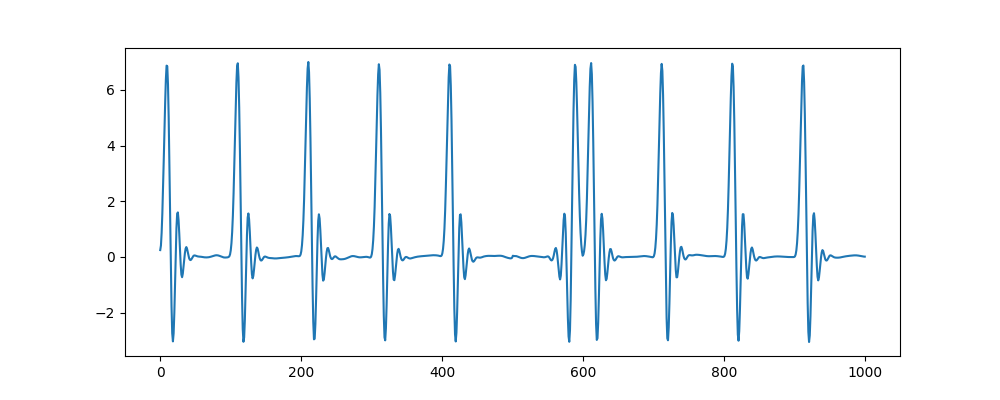
\includegraphics[width=1\linewidth]{Figures/gutenTAG_anomalies/pattern-ecg.png}
    \caption{Pattern-ecg anomaly (αναπαραγωγή από \cite{10.14778/3554821.3554873})}
    \label{figure:pattern-ecg}
    \end{figure}
    \item  \strong{Pattern Shift}: Αφορά την χρονική μετατόπιση του μοτίβου της χρονοσειράς (Σχήμα \ref{figure:pattern-shift}). 
    \begin{figure}[h]
    \centering
    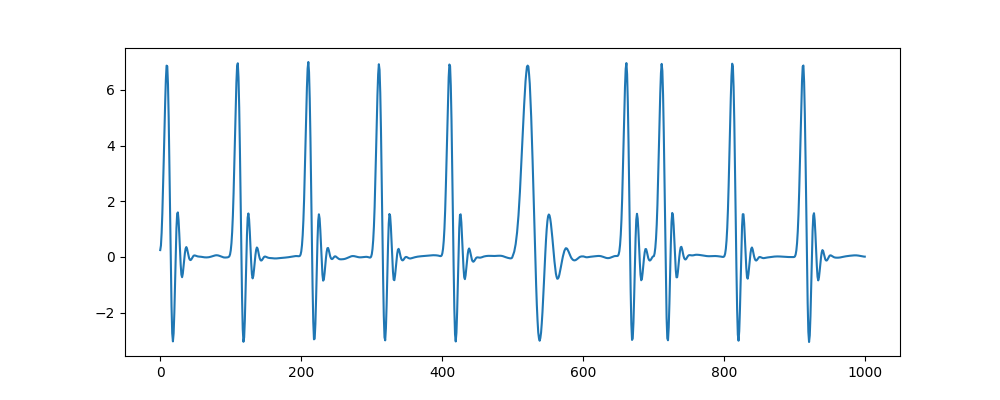
\includegraphics[width=1\linewidth]{Figures/gutenTAG_anomalies/pattern-shift.png}
    \caption{Pattern-shift anomaly (αναπαραγωγή από \cite{10.14778/3554821.3554873})}
    \label{figure:pattern-shift}
    \end{figure}
    \item \strong{Platform}: Για κάποιο χρονικά διάστημα, η χρονοσειρά "παγώνει" και έπειτα συνεχίζει κανονικά (π.χ. θα μπορούσαμε να το προσομοιάσουμε με την στιγμή που η καρδιά ενός ασθενή σταματάει να δουλεύει για κάποια δευτερολέπτα, ο ασθενής επαναφέρεται και η καρδιά δουλεύει πάλι κανονικά) (Σχήμα \ref{figure:platform}).
    \begin{figure}[h]
    \centering
    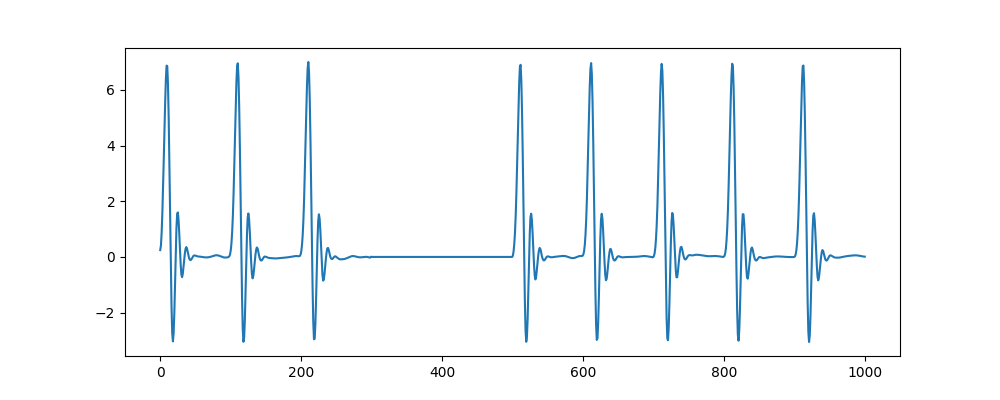
\includegraphics[width=1\linewidth]{Figures/gutenTAG_anomalies/platform.png}
    \caption{Platform anomaly (αναπαραγωγή από \cite{10.14778/3554821.3554873})}
    \label{figure:platform}
    \end{figure}
    \item \strong{Trend}: Αφορά σε μία αυξανόμενη ή μειούμενη τάση στην χρονοσειρά (Σχήμα \ref{figure:trend}).
    \begin{figure}[h]
    \centering
    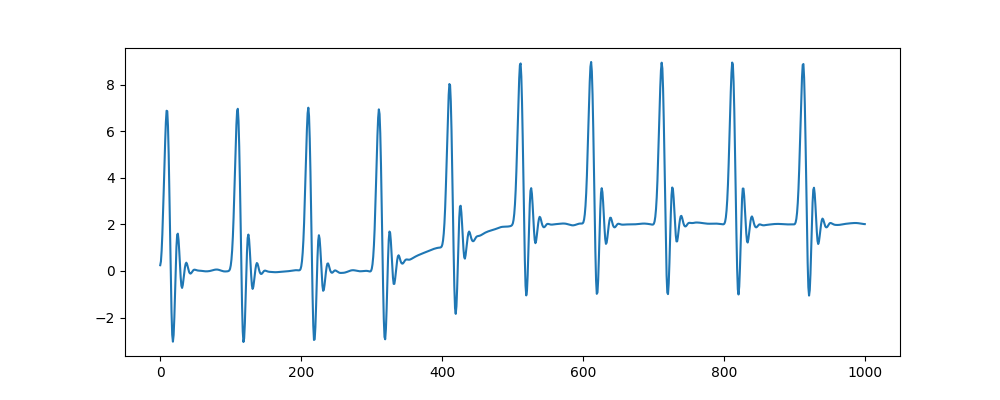
\includegraphics[width=1\linewidth]{Figures/gutenTAG_anomalies/trend.png}
    \caption{Trend anomaly (αναπαραγωγή από \cite{10.14778/3554821.3554873})}
    \label{figure:trend}
    \end{figure}
    \item \strong{Variance}: Αφορά στην μεταβολή του επίπεδου θορύβου για μία χρονική περίοδο της χρονοσειράς (Σχήμα \ref{figure:variance}).
    \begin{figure}[h]
    \centering
    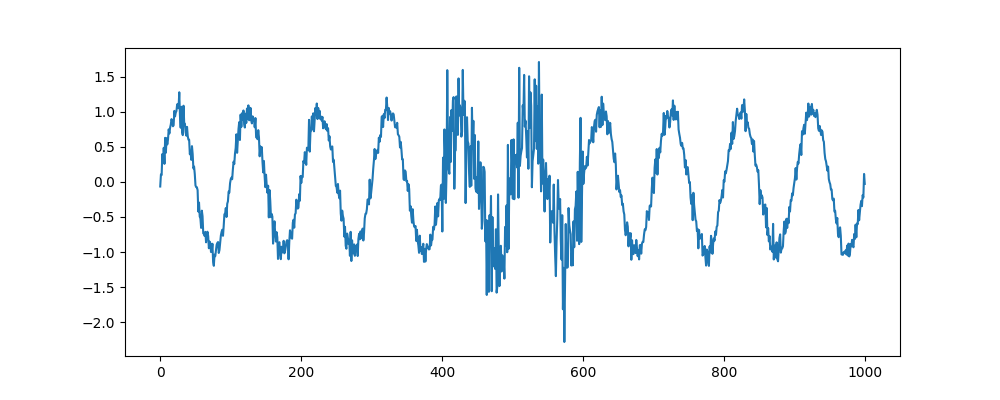
\includegraphics[width=1\linewidth]{Figures/gutenTAG_anomalies/variance.png}
    \caption{Variance anomaly (αναπαραγωγή από \cite{10.14778/3554821.3554873})}
    \label{figure:variance}
    \end{figure}
    \item \strong{Mode Correlation}: Αφορά στην αλλαγή της συμπεριφοράς μίας υπακολουθίας για το διάστημα που κρατάει η ανωμαλία (Σχήμα \ref{figure:mode-correlation}).
    \begin{figure}[h]
    \centering
    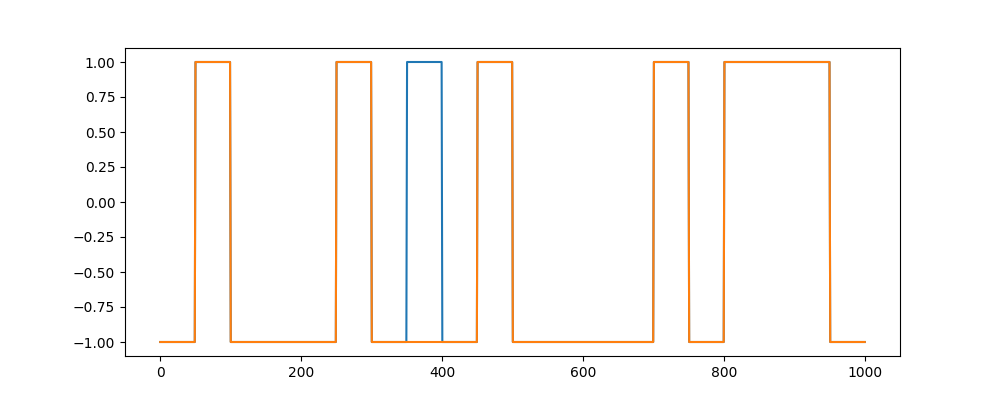
\includegraphics[width=1\linewidth]{Figures/gutenTAG_anomalies/mode-correlation.png}
    \caption{Mode correlation anomaly (αναπαραγωγή από \cite{10.14778/3554821.3554873})}
    \label{figure:mode-correlation}
    \end{figure}
\end{itemize}

Είναι πολύ πιθανό, σε χρονοσειρές πραγματικών δεδομένων, να παρατηρηθούν παραπάνω από ένας τύπος ανωμαλιών, ή ακόμα και συνδυασμοί αυτών. Τέτοια παραδείματα φαίνονται στο \ref{figure:anomalies_combined}. Στην (d.1) για παράδειγμα, μπορούμε να παρατηρήσουμε ένα \emph{point anomaly}, το \verb|A2| και ένα \emph{collective anomaly}, την υπακολουθία \verb|A1|. 

\begin{figure}[h]
    \centering
    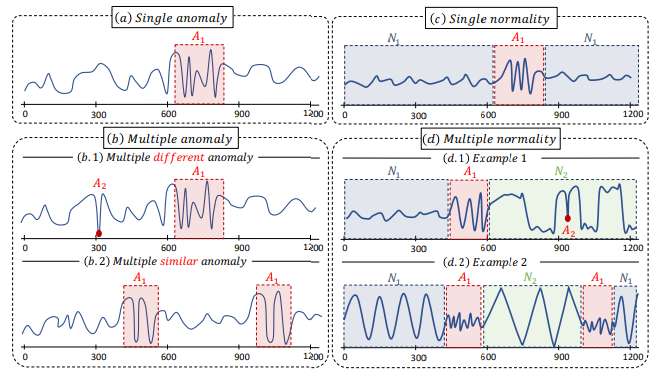
\includegraphics[width=0.7\linewidth]{Figures/anomalies_combined.png}
    \caption{Χρονοσειρές με διαφορετικούς τύπους ανωμαλιών (αναπαραγωγή από \cite{paparrizos2022tsb})}
    \label{figure:anomalies_combined}
\end{figure}



\section{Μεμονωμένοι Αλγόριθμοι Σύγκρισης}

Σε αυτό το σημείο, θα κάνουμε μία σύντομη αναφορά στους αλγορίθμους που αναφέρθηκαν στο \ref{purpose} και θα χρησιμοποιηθούν στην εργασία. Θα αναφερθεί ο τρόπος λειτουργίας τους, τα πλεονεκτήματα και τα μειονεκτήματά τους, πώς συνδέονται με την ανίχνευση ανωμαλιών, και πως οι υπερπαράμετροί τους επηρεάζουν την απόδοσή τους.

\subsection{Isolation Forest}
Οι περισσότεροι αλγόριθμοι ανίχνευσης ανωμαλιών, δημιουργούν ένα μοτίβο κανονικών δεδομένων και έπειτα, τα σημεία τα οποία αποκλίνουν από αυτό το μοτίβο, τα χαρακτηρίζουν ως ανωμαλίες. Αυτή η τεχνική έχει 2 αδυναμίες.
\begin{itemize}
    \item Πρώτον, ο αλγόριθμος είναι βελτιστοποιημένος ώστε να βρίσκει κανονικές συμπεριφορές, και όχι ανωμαλίες, οπότε μπορεί να μην είναι τόσο αποτελεσματικός στην ανίχνευση ανωμαλιών.
    \item Δεύτερον, οι περισσότερες μεθόδοι περιορίζονται σε χαμηλές διαστάσεις δεδομένων, ή και μικρό όγκο δεδομένων, λόγο της υπολογιστικής πολυπλοκότητας που απαιτείται.
\end{itemize}
Αντιθέτως, ο \emph{iForest} ακολουθεί μία διαφορετική τακτική, στοχοποιεί τις ανωμαλίες, αξιοποιώντας 2 βασικές ιδιότητες των ανωμαλιών.
\begin{itemize}
    \item Πρώτον, οι ανωμαλίες αποτελούν την μειονότητα των δεδομένων.
    \item Δεύτερον, έχουν χαρακτηριστικά τα οποία διαφέρουν πολύ από τα κανονικά δεδομένα.
\end{itemize}
Επειδή οι ανωμαλίες απομονώνονται ευκολότερα από τα κανονικά δεδομένα, βρίσκονται πιο κοντά  στην ρίζα του δένδρου. Στο
σχήμα \ref{figure:iForest1}(a), παρατηρούμε πως το σημείο $x_i$ απαιτεί περισσότερες διχοτομήσεις για να απομονωθεί, σε αντίθεση με το σημείο $x_0$, όπως φαίνεται στο \ref{figure:iForest1}(b). Επίσης στο σχήμα \ref{figure:iForest1}(c), παρατηρούμε πως η μέση απόσταση των σημείων $x_0$ και $x_i$ από την ρίζα του δένδρου, σταθεροποιείται, με μικρό αριθμό δένδρων ($n\approx10$), γεγονός που αποδυκνύει πως ο \emph{iForest} δεν απαιτεί μεγάλο αριθμό δέδρων για να συγκλίνει σε ένα καλό αποτέλεσμα.
\begin{figure}
    \centering
    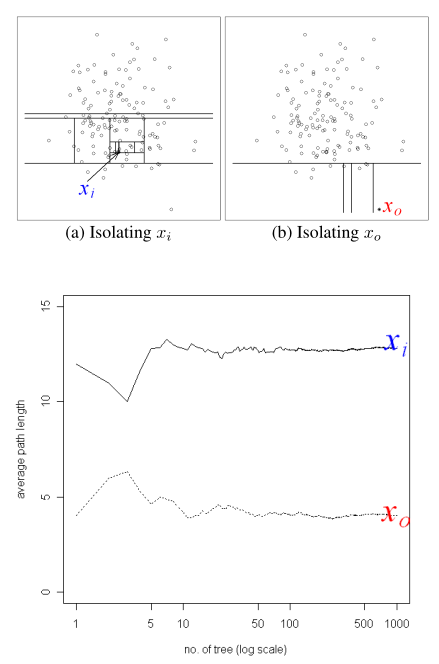
\includegraphics[width=1\linewidth]{Figures/iForest1.png}
    \caption{(a) Απομόνωση κανονικού σημείου $x_i$ (b) Απομόνωση ανώμαλου σημείου $x_0$ (c) Μέση απόσταση σημείων $x_0$ και $x_i$ από ρίζα δένδρου, με αυξανόμενο αριθμό δένδρων (αναπαραγωγή από \cite{liu2008isolation})}
    \label{figure:iForest1}
\end{figure}

Εκτός από τα παραπάνω, ο \emph{iForest} διαφέρει με τους υπόλοιπους αλγορίθμους ανίχνευσης ανωμαλιών και στα παρακάτω:
\begin{itemize}
    \item Τα χαρακτηριστικά του, του επιτρέπουν να χτίζει μόνο ένα μερικό δένδρο, το οποίο είναι αρκετό για να απομονώσει τις ανωμαλίες. Επίσης δεν χρειάζεται όλα τα δεδομένα, παρά μόνο ένα δείγμα, κάτι το οποίο βοηθάει και στην αντιμεώπιση των φαινομένων του \\ \emph{\strong{swamping}} και του \emph{\strong{masking}}.
    \begin{itemize}
        \item \emph{\strong{Swamping}}: Ονομάζεται το φαινόμενο, όπου κανονικά σημεία χαρακτηρίζονται ως ανωμαλίες. Συμβαίνει όταν τα κανονικά σημεία βρίσκονται κοντά σε ανωμαλίες.
        \item \emph{\strong{Masking}}: Ονομάζεται το φαινόμενο, όπου πολλά ανώμαλα σημεία δημιουργούν μεταξύ τους ένα cluster, δημιουργόντας την ψευδαίσθηση ενός κανονικού μοτίβου και καθιστόντας δύσκολη την ανίχνευσή τους.
    \end{itemize}
    \item Δεν χρειάζεται να υπολογίσει αποστάσεις ή πυκνότητες, άρα είναι επεκτάσιμος σε μεγάλους όγκους δεδομένων.
    \item Έχει γραμμική χρονική πολυπλοκότητα και χαημλές απαιτήσεις σε μνήμη.
    \item Τέλος είναι επεκτάσιμος σε μεγάλα σετ δεδομένων με πολλές διαστάσεις. 
\end{itemize}

Οι \emph{\strong{υπερπαράμετροι}} του \emph{iForest} είναι ο αριθμός των δένδρων $t$ που θα δημιουργηθούν και o αριθμός των δειγμάτων δεδομένων $\psi$ που θα χρησιμοποιήσουμε για κάθε δένδρο. Σύμφωνα με τους δημιουργούς του \emph{iForest} \cite{liu2008isolation} μετά από δοκιμές που έγιναν, παρατηρήθηκε ότι για $\psi=256$ και $t=100$, δεν υπήρχε μεγάλη βελτίωση του αλγορίθμου στην ανίχνευση ανωμαλιών.

Για την εφαμρογή του \emph{iForest} σε χρονοσειρές, οι δημιουργοί του \emph{TSB-UAD} \cite{paparrizos2022tsb} χρησιμοποίησαν και μία τεχνική συρόμενου παραθύρου, με σκοπό να εξάγουν υπακολουθίες, όπου ο κλασσικός \emph{iForest} χτίζει τα δένδρα του πάνω σε αυτές της υπακολουθίες. Έτσι προκύπτει μία νέα υπερπαράμετρος προς ρύθμιση, το μήκος του παραθύρου $L$.

\subsection{NormA}
Ο \emph{NormA}\cite{boniol2021unsupervised} είναι ένας αλγόριθμος, ο οποίος χρησιμοποιείται κυρίως όταν θέλουμε να ανιχνεύσουμε ανώμαλες υπακολουθίες μέσα σε μία χρονοσειρά. Οι περισσότεροι αλγόριθμοι οι οποίοι προσπαθούν να εντοπίσουν ανώμαλες υπακολουθίες εντός χρονοσειρών, συνήθως χαρακτηρίζουν ως ανώμαλη την υπακολουθία που έχει την μεγαλύτερη απόσταση από τον πλησιέστερο γείτονά της. Αντιθέτως ο \emph{NormA} λειτουργεί διαφορετικά, πρώτα βίσκει ένα μοντέλο το οποίο αντικατοπτρίζει την φυσιολογική συμπεριφορά της χρονοσειράς, το οποίο ονομάζει \emph{Normal Model - NN} και έπειτα ορίζει ως ανώμαλες, αυτές που απέχουν περισσότερο από αυτό το μοντέλο.

Ένα πρόβλημα το οποίο παρουσιάζεται συχνά στην παραπάνω μέθοδο, είναι όταν μία ανώμαλη υπακολουθία εμφανίζεται μέσα στις χρονοσειρές αρκετές φορές, τόσες ώστε να θεωρείται πλέον ως κανονική. Χαρακτηριστικό παράδειγμα είναι οι αρρυθμίες της καρδιάς ένός ασθενή. Μία τέτοια συμπεριφορά θα μπορούσε να δημιουργήσει cluster από υπακολουθίες αρρυθμιών, και να θεωρούνται πλέον ως κανονικές.

Για να δημιουργήσει το \emph{Normal Model} και να μπορεί να χαρακτηρίζει ως κανονικές ή ανώμαλες τις υπακολουθίες, ο \emph{NormA} δημιουργεί cluster από κανονικές πακολουθίες, δίνοντας στο κάθε cluster ένα βάρος $w_i$, το οποίο δηλώνει πόσο φυσιολογικό είναι το κάθε cluster. Για τον υπολογισμό του βάρους, ο αλγόριθμος βασίζεται σε 3 χαρακτηριστικά:
\begin{itemize}
    \item \emph{\strong{Συχνότητα}}: Δηλώνει πόσο συχνά εμφανίζεται αυτό το μοτίβο μέσα στην χρονοσειρά.
    \item \emph{\strong{Κάλυψη}}: Δηλώνει τι μέρος της συνολικής χρονοσειρας καλύπτει το συγκεκριμένο μοτίβο, δηλαδή σε τι ποσοστό του μήκους της χρονοσειράς εμφανίζεται.
    \item \emph{\strong{Κεντρικότητα}}: Δηλώνει πόσο κεντρικό είναι το cluster σε σχέση με τα υπόλοιπα.
\end{itemize}
Έτσι οι δημιουργοί του \emph{NormA} για να βαθμολογήσουν ένα cluster ακολουθούν τον παρακάτω τύπο:
\[
\text{Norm}(c,\mathbb{C}) = \text{Frequency}(c)^2 \times \text{Coverage}(c) \times \text{Centrality}(c,\mathbb{C})
\]
Για να επιλεγούν οι υποψήφιες υπακολουθίες για τη δημιουργία του \emph{Normal Model}, υπάρχουν 2 διαφορετικοί τρόποι: 
\begin{itemize}
    \item \emph{\strong{Norma-SJ}}: H πρώτη μέθοδος είναι η εξαντλητική, την οποία οι δημιουργοί την ονομάζουν \emph{NormA-SJ}. Εδώ υπολογίζεται η απόσταση της κάθε υπακολουθίας από τον πιο κοντινό γείτονά της, απορρίπτοντας αυτές με την μεγαλύτερη απόσταση, καθώς είναι πιο πιθανό να είναι ανωμαλίες. Το μειονέκτημα αυτής της μεθόδου είναι πως έχει τετραγωνική χρονική πολυπλοκότητα σε σχέση με το μέγεθος της χρονοσειράς.
    \item \emph{\strong{NormA-smpl}} Στην δεύτερη μέθοδο, οι ερευνητές επιλέγουν απλά ένα δείγμα από υπακολουθίες οι οποίες είναι μη επικαλυπτόμενες σύμφωνα με ένα ποσοστό $r$ (επισημαίνουν ότι $r=0.4$ είναι ιδανικό). Το πλεονέκτημα αυτής της μεθόδου είναι πως έχει γραμμική χρονική πολυπλοκότητα σε συνάρτηση με το μέγεθος της χρονοσειράς, έχοντας μικρές διαφορές στην απόδοση του αλγορίθμου. 
\end{itemize}

Ένα άλλο φαινόμενο το οποίο μπορεί να επηρεάσει αρκετά τους αλγορίθμους που προσπαθούν να ανιχνεύσουν ανώμαλες υπακολουθίες χρονοσειρών, είναι η \emph{Πολυκανονικότητα}, δηλαδή όταν υπάρχουν 2 ή περισσότερες κανονικές καταστάσεις. Εδώ οι δημιουργεί του \emph{NormA} χρησιμοποιούν μία επέκτασή του, την οποία ονομάζουν \emph{NormA-mm}, όπο μπορούν να δημιουργηθούν 2 ή παραπάνω μοντέλα ως κανονικά, ώστε να αποφεύγονται τα \emph{False Positives}.

Τέλος, ένα από τα βασικότερα πλεονεκτήματα του \emph{NormA} είναι πως απαιτεί μόνο μία υπερπαράμετρος αυτορρύθμιση, το αναμενόμενο μήκος της ανωμαλίας $l$, γεγονός που του δίνει πλεονέκτημα συγκριτικά με άλλους αλγορίθμους.


%----------------------------------------------------------------------------------------
\subsection{Matrix Profile - MP}
Ο \emph{MP} \cite{yeh2018time} δημιουργήθηκε για να λύσει ένα πρόβλημα, γνωστό ως \emph{all-pairs-similarity-search}. Πρακτικά, για κάθε δυνατή υπακολουθία μίας χρονοσειράς, προσπαθεί να εντοπίσει των πιο κοντινό της γείτονα. Ανήκει στην οικογένεια \emph{Time Series subsequences All-Pairs-Similarity-Search} (TSAPSS) αλγορίθμων, οι οποίοι συνήθως έλυναν το παραπάνω πρόβλημα με brute-force μεθόδους, είχαν τετραγωνική πολυπλοκότητα, και δεν μπορούσαν να επεκταθούν σε μεγάλα δεδομένα. Ο \emph{MP} έχει τα παρακάτω πλεονέκτηματα/χαρακτηριστικά:
\begin{itemize}
    \item \strong{Είναι ακριβής}: Δεν δίνει ψευδώς αρνητικά αποτελέσματα. Ο ισχυρισμός αυτός αναφέρεται στον υπολογιστικό τομέα της μεθόδου, καθώς ο MP υπολογίζει την απόσταση του κοντινότερου γείτονα με απόλυτη μαθηματική ακρίβεια, αποφεύγοντας προσεγγιστικές τεχνικές, που ενδέχεται να χάσουν δεδομένα. Το παραπάνω, δεν αποτρέπει περιπτώσεις όπου υπάρχουν επαναλαμβανόμενες ανωμαλίες, καθώς ο MP θα τους αποδώσει πολύ μικρό σκορ ανωμαλίας, με συνέπεια να μην μπορεί να τις αναγνωρίσει ως ανωμαλίες.
    \item \strong{Είναι απλός και δεν απαιτεί ρύθμιση παραμέτρων}
    \item \strong{Δεν απαιτεί πολύ χώρο αποθήκευσης}: Απαιτεί μόνο $O(n)$ χώρο, σε αντίθεση με άλλους αλγορίθμους που απαιτούν $O(n^2)$.
    \item \strong{Είναι \emph{anytime} αλγόριθμος}: Μπορεί να διακοπεί ανά πάσα στιγμή, και να επιστρέψει τα καλύτερα αποτελέσματα μέχρι εκείνη την στιγμή.
    \item \strong{Είναι \emph{αυξηντικός}}: Σε συνεχόμενη ροή δεδομένων, δεν απαιτείται η επανεκτέλεσή του, παρά μόνο η ενημέρωση των αποτελεμσάτων του, με βάση τα καινούργια δεδομένα.
    \item \strong{Δεν απαιτεί ορισμού κατωφλιού ομοιότητας/απόστασης}: Σε αντίθεση με 'αλλους αλγορίθμους, δεν απαιτεί να οριστεί κάποιο κατώφλι ομοιότητας/απόστασης, καθώς εκμεταλλεύεται τα \emph{full joins}.
    \item \strong{Μπορεί να εκμεταλλευτεί το hardware}: Είναι σχεδόν πλήρος παραλληλοποιήσιμος, και μπορεί να εκμεταλλευτεί το hardware, όπως πολλαπλούς πυρήνες, ή ακόμα και GPU, ακόμα και κατανεμημένα συστήματα.
    \item \strong{Έχει σταθερή χρονική πολυπλοκότητα, η οποία ΔΕΝ είναι ανάλογη του μήκους της υπακολουθίας}.
    \item \strong{Απαιτεί ντετερμινιστικό χρόνο για να ολοκληρωθεί}: Ένα εξαιρετικά σημαντικό χαρακτηριστικό το οποίο δεν είναι καθόλου συνηθισμένο σε αλγόριθμους αυτού του πεδίου. Δεδομένου μόνο του μήκους της χρονοσειράς, μπορεί να προβλέψει με ακρίβεια τον χρόνο εκτέλεσης που θα χρειαστεί για να ολοκληρωθεί.
\end{itemize}

Για να κατανοήσει κανείς τον \emph{MP}, πρέπει πρώτα να ορίστεί η έννοια του \emph{Distance Profile}. Δεδομένης μίας συγκεκριμένης υπακολουθίας, το \emph{Distance Profile} είναι ένα διάνυσμα στο οποίο αποθηκεύεται η ευκλείδια απόσταση, εφόσον έχει προηγηθεί Ζ-κανονικοποίηση, μεταξύ της συγκεκριμένης υπακολουθίας και όλων των άλλων υπακολουθιών. Έτσι το \emph{Matrixe Profile}, είναι στην ουσία ένα μονοδιάστατο διάνυσμα, στο οποίο αποθηκεύεται για κάθε υπακολουθία, η ελάχιστη απόστασή της, από το \emph{Distance Profile} της, δηλαδή την απόστασή της από τον πιο κοντινό γείτονά της. Ταυτόχρονα, σε ένα άλλο διάνυσμα, το οποίο ονομάζεται \emph{Matrix Profile Index}, αποθηκεύεται και ο δείκτης της κάθε υπακολουθίας προς τον πιο κοντινό γείτονά της.

Έτσι, μπορούμε να χρησιμοποιήσουμε τον \emph{MP} για δύο αντίθετα προβλήματα:
\begin{itemize}
    \item \strong{Motif Discovery}: Εντοπισμός των πιο παρόμοιων ζευγών υπακολουθιών. Αυτά τα σημεία, είναι συνεχόμενα και χαμηλά σε ένα διάγραμμα.
    \item \strong{Discord Discovery}: Εντοπισμός των πιο διαφορετικών ζευγών υπακολουθιών, δηλαδή των ανωμαλιών. Αυτά τα σημεία, σε αντίθεση με πριν, είναι απότομα και δημιουργούν κορυφές σε ένα γράφημα. Όπως φαίνεται και στο σχήμα \ref{figure:MP}, το σημείο που εντοπίστηκε η ανωμαλία στο ηλεκτροκαρδιοφγράφημα, αντιστοιχεί στο σημείο με την μεγαλύτερη κορυφή στο διάγραμμα του \emph{MP}.
\end{itemize}

\begin{figure}
    \centering
    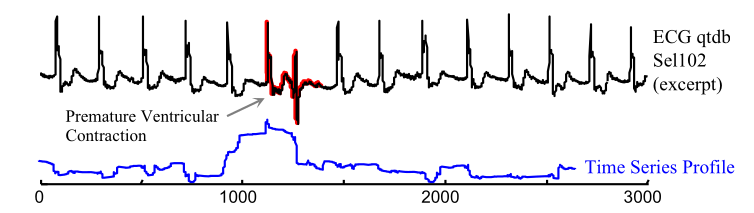
\includegraphics[width=0.8\linewidth]{Figures/MP_anomaly_detection.png}
    \caption{Ανχίχνευση ανωμαλιών με τον \emph{Matrix Profile} (αναπαραγωγή από \cite{yeh2018time})}
    \label{figure:MP}
\end{figure}

Για τον υπολογισμό του \emph{Distance Profile}, ο \emph{MP} χρησιμοποιεί τον αλγόριθμο \emph{MASS}, ο οποίος βασίζεται στον \emph{Fast Fourier Transform} (FFT). Με αυτόν τον τρόπο, η χρονική πολυπλοκότητα του υπολογισμού του \emph{Distance Profile} είναι $O(nlog n)$.
Έπειτα, για τον υπολογισμό ολόκληρου του \emph{Matrix Profile}, υπάρχουν 3 διαφορετικές μεθόδοι που ανέπτυξαν οι ερευνητές του \emph{MP}:
\begin{itemize}
    \item \emph{\strong{STAMP} (Scalable Time series Anytime Matrix Profile)}: Αυτός ο αλγόριθμος, υπολογίζει το \emph{Distance Profile} για κάθε υπακολουθία με τυχαία σειρά. Έτσι, ο χρήστης μπορεί ανά πάσα στιμγή να διακόψει την εκτέλεση του αλγορίθμου, και να πάρει μία προσέγγιση του \emph{Matrix Profile}. Η χρονική πολυπλοκότητα ανέρχεται σε $O(n^2log n)$, αλλά με βάση τα πειράματα των δημιουργών, η τελική χρονική πολυπλοκότητα είναι $O(n^2)$. Μία πιθανή εξήγηση για το παραπάνω συμβάν, είναι πως επειδή ο \emph{FFT} είναι πολύ σημαντικός σε πάρα πολλές εφαρμογές, είναι υπερβολικά πολύ βελτιστοποιημένος.
\item  \emph{\strong{STOMP} (Scalable Time series Ordered-search Matrix Profile)}: Είναι μία πιο γρήγορη παραλλαγή του \emph{STAMP} αν ο χρήστης διατίθεται να θυσιάσει το χαρακτηριστικό του \emph{anytime}. Η παραλλαγή αυτή, σαρώνει την χρονοσειρά με αυστηρή σειρά, από την αρχή προς το τέλος. Αυτό είναι σημαντικό, καθώς οι δημιουργοί του \emph{MP} παρατήρησαν πως για να βρεις το εσωτερικό γινόμενο $QT_{j,i}$ όπου $Q:$ η προς εξέταση υπακολουθία, μεταξύ 2 μετατοπισμένων υπακολουθιών κατά μία θέση, αρκεί να υπολογίσεις το προηγούμενο εσωτερικό γινόμενο $QT_{j-1,i-1}$ αφαιρόντας το παλαιότερο σημείο και προσθέτοντας το νεότερο, σε μόλις $O(1)$. Έτσι, η τελική χρονική πολυπλοκότητα του \emph{STOMP} είναι $O(n^2)$.
\item \emph{\strong{STOMPI} (Stomp Incremental)}: Παραλλαγή του \emph{STOMP}, η οποία δουλεύει για ροές δεδεομένων. Δεν επαναυπολογίζει ολόκληρο τον \emph{MP} από την αρχή, παρά μόνο ενημερώνει τα αποτελέσματα με βάση τα καινούργια δεδομένα. Η χρονική πολυπλοκότητα του \emph{STOMPI} είναι $O(n)$, όπου $n$ είναι το μήκους της μέχρι τώρα ακολουθίας. Αυτό συνεπάγεται, πως για κάθε σημείο που προστίθεται, ο αλγόριθμος γίνεται όλο και πιο αργός. Άρα ο καλύτερος τρόπος για να εξετάσουμε την απόδοσή του, είναι να μελετήσουμε τον \strong{Μέγιστο Χρονικό Ορίζοντα (ΜΗΤ)}. Θεωρόντας ένα παράδειγμα, όπου ένα dataset ενημερώνεται κάθε 8 δευτερόλεπτα, ο \emph{STOMPI} θα μπορούσε να τρέξει για 25 χρόνια. Αυτή η εκτίμηση που δίνουν οι ερευνητές είναι, χωρίς να συμπεριλάβουμε τις βελτιστοποιήσης που συμβαίνουν συνεχώς στο hardware.
\end{itemize}

Αν και στις περισσότερες περιπτώσεις, οι παραπάνω αλγόριθμοι θα μας κάλυπταν, υπάρχουν και κάποιοι κλάδοι, όπως αυτός των σεσμολόγων, οι οποίοι θα ήθελαν να έχουν απεριόριστο όριο στα δεδομένα τους. Για τέτοιους σκοπούς συγκεκριμένα, οι ερευνητές μετέφεραν τον \emph{STAMP} σε \emph{CUDA C++}, εκμεταλλευόμενοι της τεράστιες δυνατότητες για παράλληλισμό των επεξεργαστών της \emph{NVDIA}.

Ένα από τα πλεονεκτήματα που αναφέραμε προηγουμένος, είναι πως μπορούμε να γνωρίζουμε εκ των προτέρων, πόσο χρόνο θα χρειαστεί για να εκτελέσουμε τον \emph{MP}. Αυτό το επιτυγχάνουμε κάνοντας αρχικά ένα δοκιμαστικό έλεγχο στο μηχάνημά μας, υπολογίζοντας πόσο χρόνο $\delta$ θα κάνει για να υπολογίσει το \emph{MP} σε μία τυχαία χρονοσειρά μεγέθους $n$. Έπειτα για μία καινούργια χρονοσειρά μεγέθους $n_{new}$
το καινούργιο $\delta_{new}$ υπολογίζεται ως εξής:
$$\delta_{new} = \frac{\delta}{n^2} \times n_{new}^2$$

\begin{figure}
    \centering
    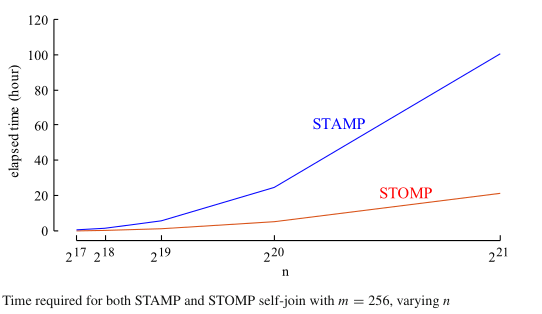
\includegraphics[width=0.8\linewidth]{Figures/stamp_stomp_varryingN.png}
    \caption{(αναπαραγωγή από \cite{yeh2018time})}
    \label{figure:STAMP-STOMP-VarN}
\end{figure}

Σημαντικό είναι να δούμε, τους απαιτούμενους χρόνους για τον \emph{STAMP} και τον \emph{STOMP}, όταν κρατάμε σταθερή την μία από τις 2 παραμέτρους ($n,m$).Παρατηρούμε στο σχήμα \ref{figure:STAMP-STOMP-VarN} πως ο \emph{STOMP} έχει σημαντικά καλύτερους χρόνους εκτέλεσης από τον \emph{STAMP} όσο μεγαλώνει το μέγεθος της χρονοσειράς. Το πιο σημαντικό όμως είναι, όπως φαίνεται στο σχήμα \ref{figure:STAMP-STOMP-VarM}, πως και οι 2 αλγόριθμοι, είναι σχεδόν σταθεροί ανεξαρτήτως του μεγέθους $m$ της υπακολουθίας. Μάλιστα φαίνεται να υπάρχει μία ελαφρώς φθίνουσα πορεία, όσο μεγαλώνει το $m$. Αυτό συμβαίνει διότι όσο μεγαλώνει το $m$, ο αριθμός των συγκρίσεων γίνεται όλο και μικρότερος.  

\begin{figure}
    \centering
    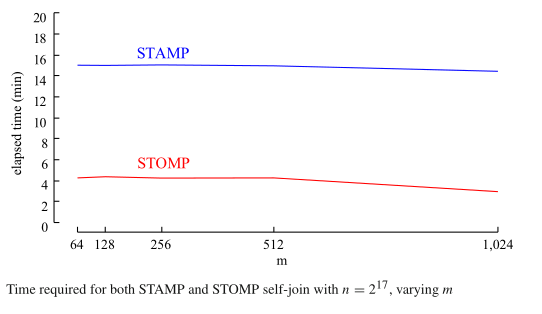
\includegraphics[width=0.8\linewidth]{Figures/stamp_stomp_varryingM.png}
    \caption{(αναπαραγωγή από \cite{yeh2018time})}
    \label{figure:STAMP-STOMP-VarM}
\end{figure}

Γενικά ο \emph{MP}, είναι μία από τις ταχύτερες/ακριβέστερες μεθόδους ανίχνευσης μοτίβων/ανωμαλιών, η οποία παρουσιάζει όμως ένα αδύνατο σημείο, το οποίο τονίζουν και οι ερευνητές του. Όταν υπάρχουν επαναλαμβανόμενες ανωμαλίες μέσα στα δεδομένα, μπορεί να θεωρήσει αυτά τα μοτίβα ως φυσιολογικά, διότι βασίζεται αυστηρά στην απόσταση του 1ου κοντινότερου γείτονα. Για παράδειγμα, αν σε εά ηλεκτροκαρδιογράφημα, ένας ασθενής έχει επαναλαμβανόμενες αρυθμίες, αυτές θα σημανθούν ως κανονικές, κάτι το οποίο δεν είναι επιθυμητό. Το παραπάνω γεγονός επιβεβαιώθηκε και από τους δημιουργούς του \emph{TSB-UAD}.

\subsection{POLY}
Ο αλγόριθμος \emph{POLY} \cite{li2007unifying} για την εύρεση ανωμαλιών σε χρονοσειρές, σε αντίθεση με άλλους αλγορίθμους οι οποίοι απαιτούν να είναι γνωστό εκ των προτέρων του τύπου του μοντέλου της χρονοσειράς ή είναι αρκετά ευαίσθητοι σε υπερπαράμετρους, αντιμετωπίζει το πρόβλημα με διαφορετική προσέγγιση. Χρησιμοποιόντας την τεχνική της Τοπικής Πολυωνυμικής Προσαρμογής (Local Polynomial Fitting), αποφεύγοντας την ανάγκη για παραμέτρους, και με την βοήθεια του \emph{Ασαφή Διαχωρισμού} και της \emph{Θεωρίας Λήψης Αποφάσεων}, μπορεί να εντοπίσει ανωμαλίες σε online χρονοσειρές, αλλά και σημεία αλλάγης (change points).

Οι ανωμαλίες και τα σημεία αλλαγής, μπορούν να περιγραφούν μέσω της συνολικής κανονικότητας του συστήματος (holistic regularity). Έτσι, οι δημιουργοί του \emph{POLY} ορίζουν σαν ανωμαλία, ένα σημείο το οποίο αποκλίνει σημαντικά από την συνολική κανονικότητα της χρονοσειράς, ενώ εά σημείο αλλαγής, αποτελεί το χρονικό σημείο από το οποίο και μετά, αλλάζει ολόκληρη η συνολική κανονικότητα της χρονοσειράς.

Για να ποσοτικοποιήσουν μαθηματικά αυτήν την συμπεριφορά, εξετάζουν δύο δύο δεσμευμένες πυκνότητες πιθανότητας για κάθε σημείο $x_t$ της χρονοσειράς:
\begin{itemize}
    \item \strong{Forward Conditional Density}: η οποία υπολογίζεται βάσει ενός παραθύρου δεδομένων του παρελθόντος $p(x_t|x_{t-L},...,x_{t-1})$.
    \item \strong{Backward Conditional Density}: η οποία υπολογίζεται βάσει ενός παραθύρου δεδομένων του μέλλοντος $p(x_t|x_{t+1},...,x_{t+L})$.
\end{itemize}

Οι παραδοσιακές μεθόδοι, προσπαθούσαν να υπολογίσουν αυτές τις πυκνότητες, προσαρμόζοντας τα δεδομένα τους σε αυστηρά καθολικά παραμετρικά μοντέλα. Κάτι τέτοιο όμως δεν είναι δυνατόν για χρονοσεριές, και έτσι οι δημιουργοί του \emph{POLY} υιοθέτησαν την τεχνική της Τοπικής Πολυωνυμικής Προσαρμογής, όπου για κάθε χρονικό σημείο, απομονώνεται μόνο ένα μικρό τοπικό παράθυρο, όπου ο αλγόριθμος προσπαθεί να ταιριάξει μία απλή τοπική καμπύλη. Βάση αυτής της καμπύλης ο αλγόριθμος υπολογίζει ποιά θα έπρεπε να είναι αναμενόμενη τιμή του σημείου που εξετάζεται.

Έχοντας πλέον την δυνατότητα να προβλέψει την αναμενόμενη τιμή κάθε σημείου μέσω των τοπικών πολυωνύμων, ο αλγόριθμος πρέπει να αποφασίσει αν ενα σημείο είναι ανώμαλο/σημείο αλλαγής ή όχι. Αρχικά, για κάθε σημείο υπολογίζει δύο βαθμολογίες, την \emph{Forward Score} και την \emph{Backward Score}, όπου είναι ίσες με το τετράγωνο της διαφοράς μεταξύ της πραγματικής και της εκτιμώμενης τιμής του σημείου, διαιρούμενη με την διακύμανση των δεδομένων του παραθύρου.

Ωστόσο, η απόφαση για το αν ένα σημείο είναι ανώμαλο/σημείο αλλαγής, δεν γίνεται απλά με βάση κάποιο κατώφλι, αλλά υιοθετείται μία διαφορετική λογική, η οποία πηγάζει από τα \emph{Ασαφή Σύνολα}. Το σύστημα χρησιμοποιώντας τις αρχικές βαθμολογίες, και δύο σταθερές ανοχής, δεν απορρίπτει ούτε αποδέχεται απόλυτα εά σημείο, αλλά υπολογίζει τον βαθμό συμμετοχής του, σε τέσσερις διαφορετικές καταστάσεις, όπως φαίνονται παρακάτω:
\begin{itemize}
    \item \strong{FNormalX}: Το σημείο θεωρείται φυσιολογικό σε σχέση με τα δεδομένα του παρελθόντος.
    \item \strong{BNormalX}: Το σημείο θεωρείται φυσιολογικό σε σχέση με τα δεδομένα του μέλλοντος.
    \item \strong{NotFNormalX}: Το σημείο δεν θεωρείται κανονικό σε σχέση με τα δεδομένα του παρελθόντος.
    \item \strong{NotBNormalX}: Το σημείο δεν θεωρείται κανονικό σε σχέση με τα δεδομένα του μέλλοντος.
\end{itemize}

Έπειτα δημιουργούνται 2 ασαφή σύνολα:
\begin{itemize}
    \item \strong{Outlier Set}: όπου $Outlier = NotFNormalX \cap NotBNormalX$ και ανήκουν τα ανώμαλα σημεία της χρονοσειράς.
    \item \strong{Change Point Set}: όπου $Change = NotFNormalX \cap BNormalX$ και ανήκουν τα σημεία αλλαγής της χρονοσειράς.
\end{itemize}

Οι κύριες ρυθμίσεις που απαιτούνται για τον \emph{POLY} είναι το μέγεθος του παραθύρου $h$ και ο βαθμός του τοπικού πολυωνύμου $p$. Οι δημιουργού του, προτείνουν ο βαθμός του πολυωνύμου να είναι περιττός αριθμός (π.χ. $p=1$, $p=3$), καθώς από πειράματα που έκαναν, παρατήρησαν ότι προσφέρει καλύτερη προσαρμογή στα δεδομένα.Το μέγεθος του παραθύρου $h$ μπορεί να υπολογιστεί δυναμικά, όπου σαν αρχικές τιμές δίνουν $h=[X^f_{max} - X^f_{min}]/(L-1)$ για την εμπρόσθια εκτίμηση, και $h=[X^b_{max} - X^b_{min}]/(L-1)$ για την οπίσθια εκτίμηση, αναπροσαρμόζοντάς τας με έναν παράγοντα $C=1.1$, μέχρι το $MISE(h)\leq\delta$, όπου $\delta$ είναι ένα κατώφλι για το $MISE$.

